\documentclass{article}[18pt]
\usepackage[utf8]{inputenc}
\usepackage[margin=0.7in]{geometry}
\usepackage{amsmath}
\usepackage{titlesec}
\usepackage{pgfplots}
\usepackage{graphicx}
\usepackage[english]{babel}
\usepackage{fancyhdr}
\usepackage{gensymb}
\usepackage{tabularx}
\usetikzlibrary{decorations, decorations.text,positioning,quotes,arrows.meta,decorations.markings,3d,shapes,decorations.pathmorphing}
\pgfplotsset{width=10cm,compat=1.9}
\usepackage[super]{nth}
\titlespacing\section{0pt}{14pt plus 4pt minus 2pt}{0pt plus 2pt minus 2pt}
\newlength\tindent
\setlength{\tindent}{\parindent}
\setlength{\parindent}{0pt}
\renewcommand{\indent}{\hspace*{\tindent}}
\hyphenpenalty =10000
\pagestyle{fancy}
\fancyhf{}
\rhead{Sam Robbins 13SE}
\lhead{A Level Physics - Nuclear Physics}
\rfoot{Page \thepage}
\usepackage{mathtools}
\usetikzlibrary{calc,quotes,angles}
\tikzstyle{arrow} = [thick,->,>=stealth]
\begin{document}
\begin{center}
\underline{\huge Radioactivity}
\end{center}
\section{Rutherford Scattering}
\subsection{The plum pudding model}
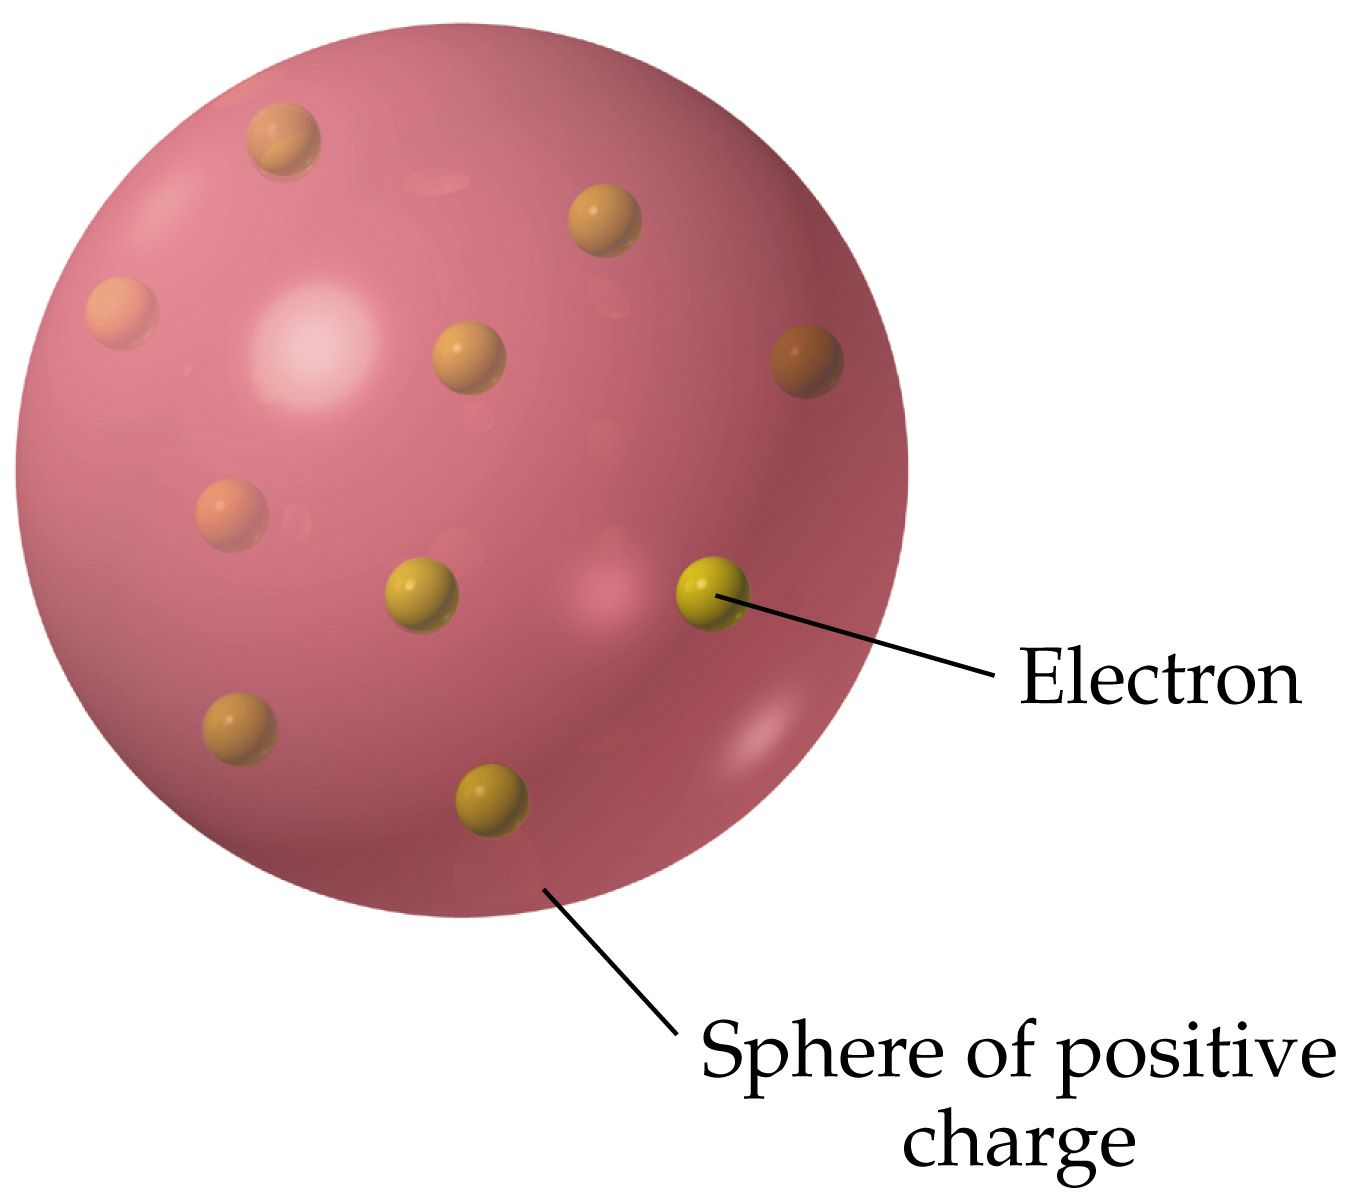
\includegraphics[width=3cm] {plum.jpg}  
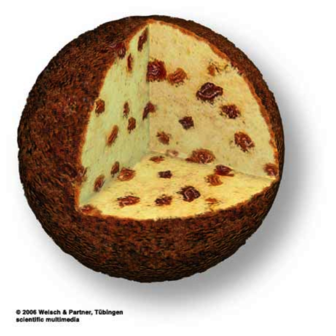
\includegraphics[width=3cm] {Plumpudding.png}
\\
The plum pudding model was the initial model of the atom, stating a sphere of positive charge with electrons embedded into it.
\subsection{Rutherford's experiment}
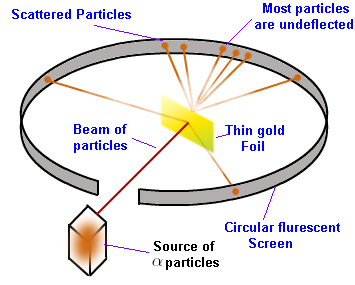
\includegraphics[width=6cm] {scatter.png}\\
Rutherford's experiment involved firing a beam of alpha particles at gold foil and measuring the paths of particles from the foil.
\begin{itemize}
\item Gold was used as it was expected to have a large nucleus
\item The screen fluoresces when collided with
\item This showed the atom was mostly empty space with a positive nucleus
\end{itemize}
\subsubsection{Results}

\begin{figure}[h]
    \centering
    \begin{minipage}{0.45\textwidth}
        \centering
        
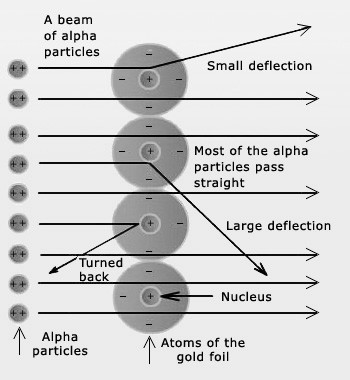
\includegraphics[width=6cm]{foil.jpg}  
    \end{minipage}\hfill
    \begin{minipage}{0.45\textwidth}
        \centering
\begin{tabularx}{\textwidth}{|X|X|}
\hline
Observation&Explanation\\
\hline
Most electrons pass all the way through&Atoms are mostly empty space\\
\hline
Some are deflected&The atom has a positive centre\\
\hline
Some are deflected by significant angles&The positive charge is condensed in a small area\\
\hline
\end{tabularx}
    \end{minipage}
\end{figure}
\subsection{Estimating the size of the nucleus}  
\subsubsection{Closest approach method}
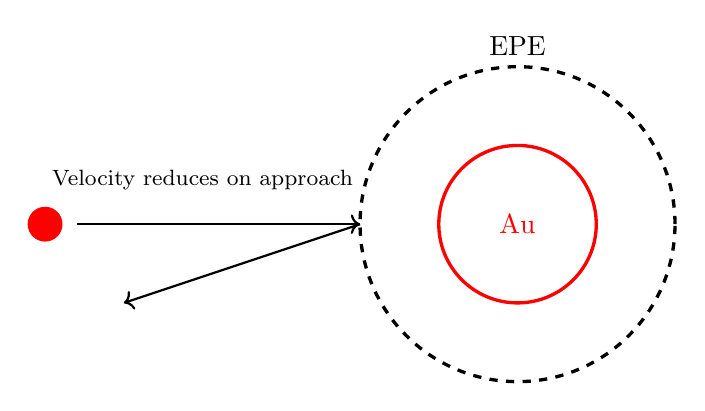
\begin{tikzpicture}
\filldraw[color=red, fill=red, very thick](0,0) circle (0.2);
\draw[thick, ->,black] (0.4,0) -- (4,0) node[above,yshift=0.3cm,xshift=-2cm] {\footnotesize{Velocity reduces on approach}};
\draw[color=red, very thick](6,0) circle (1) node[] {Au};
\draw[color=black, very thick,dashed](6,0) circle (2) node[above,yshift=2cm] {EPE};
\draw[thick, ->,black] (4,0) -- (1,-1);
\end{tikzpicture}\\
\\
KE=EPE
$$8.0\times10^{-13}=\frac{1}{4\pi\epsilon_0}\times\frac{Q_{Au}}{r}\times Q_{\alpha}$$
$$r=4.55\times10^{-14}$$
\subsubsection{Estimate from scattering data}
\begin{itemize}
\item About $\frac{1}{10,000}$ deflected through more than 90\degree
\item Foil had n layers of atoms
\end{itemize}
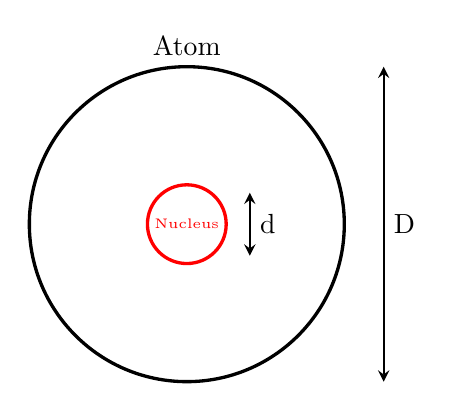
\begin{tikzpicture}
\draw[thick, stealth-stealth,black] (6.8,-0.4) -- (6.8,0.4) node[right,midway] {d} ;
\draw[color=red, very thick](6,0) circle (0.5) node[] {\tiny{Nucleus}};
\draw[color=black, very thick](6,0) circle (2) node[above,yshift=2cm] {Atom};
\draw[thick, stealth-stealth,black] (8.5,-2) -- (8.5,2) node[right,midway] {D};
\end{tikzpicture}\\
$$\frac{\frac{1}{4}\pi d^2}{\frac{1}{4}\pi D^2}=\frac{d^2}{D^2}=\frac{1}{10,000n}$$
$n=10^4$ layers
$$\frac{d^2}{D^2}=\frac{1}{10,000\times1\times10^4}$$
$$d=\frac{D}{10,000}$$
\newpage
\section{Radioactive materials}
\subsection{Sources of background radiation by most common}
\begin{enumerate}
\item Air (e.g. radon gas)
\item Medical
\item Ground and buildings
\item Food and drink
\item Cosmic rays
\item Nuclear weapons
\item Air travel
\item Nuclear power
\end{enumerate}
\subsection{Geiger M\"{u}ller tube}
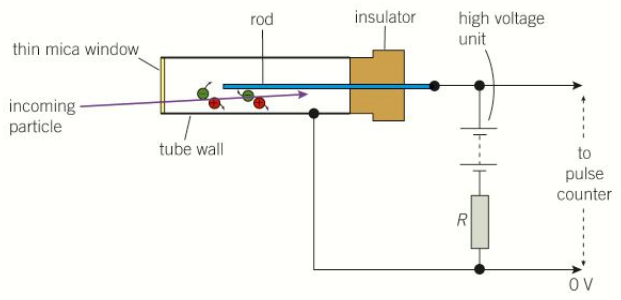
\includegraphics[width=10cm]{geiger.png}\\
When a particle of ionising radiation enters the tube, the particle ionises the gas atoms along its track. The negative ions are attracted to the rod and the positive ions to the wall. These ions cause further ionisation, creating enough ions for a current to flow. A pulse of charge passes round the circuit through resistor R, causing the voltage pulse across R which is recorded as a single count by the pulse counter\\
\\
The dead time of the tube, the time taken to regain its non conducting state after an ionising particle enters it, is typically of the order of 0.2ms.\\
\section{Radioactive decay}
\begin{tabularx}{\textwidth}{|c|X|X|X|}
\hline
&Alpha&Beta&Gamma\\
\hline
Nature&2 Protons+2 Neutrons&High speed electron or positron&High energy photon\\
\hline
Range&Up to 10cm&Up to 1m&Infinite\\
\hline 
Deflection in a magnetic field&Deflected&Opposite direction to $\alpha$ particles and more easily deflected&Not deflected\\
\hline
Absorption&Paper&Aluminium&Lead \\
\hline
Ionisation&$10^4$ ions per mm&100 ions per mm&Very weak ionising effect\\
\hline
Energy of each particle&Constant for a given source&Varies up to a maximum for a given source&Constant for a given source\\
\hline
\end{tabularx}
\newpage
\subsection{$\alpha$ Decay}
$$^{238}_{92}U\rightarrow^4_2\alpha+^{234}_{90}Th$$
\subsection{$\beta^-$ Decay}
Neutron to proton and $\beta^-$ particle
$$^{14}_6C\rightarrow^0_{-1}\beta+^{14}_7N$$
\subsection{$\beta^+$ Decay}
Proton to neutron and $\beta^+$
\subsection{Electron Capture}
Proton+Electron$\rightarrow$ Neutron
\subsection{Gamma Emission}
No change to the structure of the nucleus.\\
Often follows alpha or beta emission. Daughter nucleus can be in an excited state. It emits gamma radiation as it returns to its ground state.
\subsection{NZ Plot}
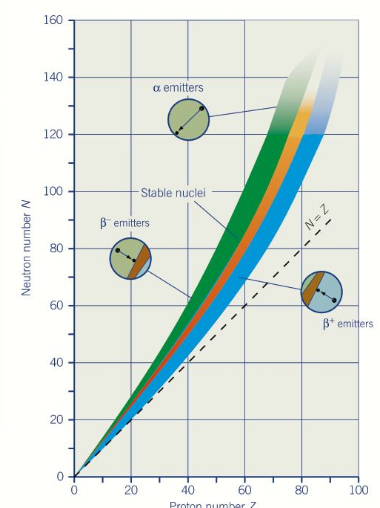
\includegraphics[width=5cm]{nz_plot.png} 
\subsection{Half life}
The half life of a radioactive substance is the time taken for half the atoms in the sample to decay.
$$\textrm{The rate of decay}\propto\textrm{The number of nuclei left}$$
$$-\frac{\Delta N}{\Delta t}\propto N$$
The LHS of this equation is called the activity and has units Bq
$$-\frac{\Delta N}{\Delta t}=\lambda N$$
The solution to this equation
$$N=N_0e^{-\lambda t}$$
This can also be written as:
$$\frac{N}{N_0}=e^{-\lambda t}$$
\subsubsection{Linking the formula to half life}
After a time, t=$T_{\frac{1}{2}}$ the fraction remaining is 0.5.
$$0.5=e^{-\lambda t}$$
$$ln(2)=\lambda t$$
$$t=\frac{\ln(2)}{\lambda}$$
$\lambda t$ is a "Pure Number". As long as the same units are used for both, you can use any unit of time.\\
\\
$\lambda$ is the fraction of nuclei decaying per unit time or the probability of an individual nucleus decaying per second.\\
As N is proportional to Activity, Mass and Count Rate N can be replaced with any of these in the formula.
\end{document}
